\section{peo\-Async\-Island\-Mig$<$ EOT $>$ Class Template Reference}
\label{classpeo_async_island_mig}\index{peoAsyncIslandMig@{peoAsyncIslandMig}}
The {\bf peo\-Async\-Island\-Mig}{\rm (p.\,\pageref{classpeo_async_island_mig})} class offers the elementary basis for implementating an asynchronous island migration model - requires the specification of several basic parameters, i.e.  


{\tt \#include $<$peo\-Async\-Island\-Mig.h$>$}

Inheritance diagram for peo\-Async\-Island\-Mig$<$ EOT $>$::\begin{figure}[H]
\begin{center}
\leavevmode
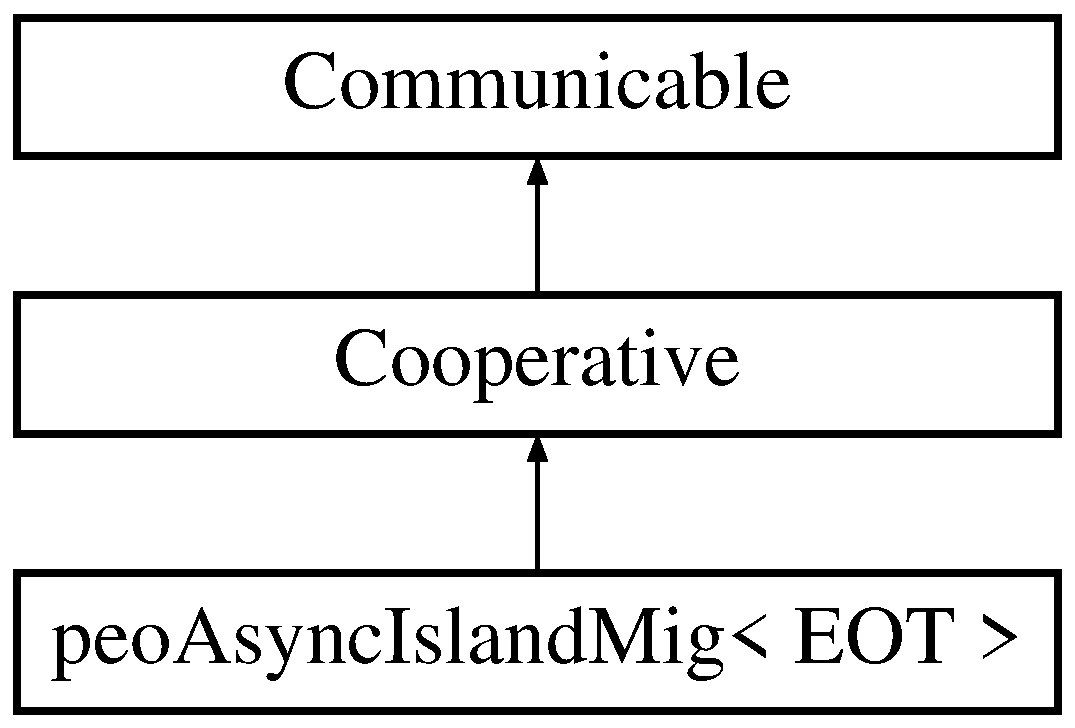
\includegraphics[height=3cm]{classpeo_async_island_mig}
\end{center}
\end{figure}
\subsection*{Public Member Functions}
\begin{CompactItemize}
\item 
{\bf peo\-Async\-Island\-Mig} (eo\-Continue$<$ EOT $>$ \&\_\-\_\-cont, eo\-Select$<$ EOT $>$ \&\_\-\_\-select, eo\-Replacement$<$ EOT $>$ \&\_\-\_\-replace, {\bf Topology} \&\_\-\_\-topology, eo\-Pop$<$ EOT $>$ \&\_\-\_\-source, eo\-Pop$<$ EOT $>$ \&\_\-\_\-destination)
\begin{CompactList}\small\item\em Constructor for the {\bf peo\-Async\-Island\-Mig}{\rm (p.\,\pageref{classpeo_async_island_mig})} class; the characteristics of the migration model are defined through the specified parameters - out of the box objects provided in EO, etc., or custom, derived objects may be passed as parameters. \item\end{CompactList}\item 
void {\bf operator()} ()
\begin{CompactList}\small\item\em Function operator to be called as checkpoint for performing the migration step. \item\end{CompactList}\item 
void {\bf pack} ()\label{classpeo_async_island_mig_6d790a5d0b6ac510cac4f61a1c0d8f16}

\begin{CompactList}\small\item\em Auxiliary function dealing with sending the emigrant individuals. There is no need to explicitly call the function. \item\end{CompactList}\item 
void {\bf unpack} ()\label{classpeo_async_island_mig_455501aee5db2bbfbae15779c8429369}

\begin{CompactList}\small\item\em Auxiliary function dealing with receiving immigrant individuals. There is no need to explicitly call the function. \item\end{CompactList}\end{CompactItemize}
\subsection*{Private Member Functions}
\begin{CompactItemize}
\item 
void {\bf emigrate} ()\label{classpeo_async_island_mig_87a4ef7d4bd30d349a801bf0f9e87c82}

\item 
void {\bf immigrate} ()\label{classpeo_async_island_mig_5a9a64ba51a696e45f91b362c39c9a64}

\end{CompactItemize}
\subsection*{Private Attributes}
\begin{CompactItemize}
\item 
eo\-Continue$<$ EOT $>$ \& {\bf cont}\label{classpeo_async_island_mig_2fc077d02ef9ea4595cfe883af0d4f83}

\item 
eo\-Select$<$ EOT $>$ \& {\bf select}\label{classpeo_async_island_mig_b1fa045094c8a411323e75b5820c80c2}

\item 
eo\-Replacement$<$ EOT $>$ \& {\bf replace}\label{classpeo_async_island_mig_b761dbd880ee32e170741ecd78da6f48}

\item 
{\bf Topology} \& {\bf topology}\label{classpeo_async_island_mig_e45e5a808a96f0853ab6ba42339fe679}

\item 
eo\-Pop$<$ EOT $>$ \& {\bf source}\label{classpeo_async_island_mig_8a502d82c773033e274dca932fc2d4ee}

\item 
eo\-Pop$<$ EOT $>$ \& {\bf destination}\label{classpeo_async_island_mig_e407f411d08ae7d96992603c145a7e43}

\item 
std::queue$<$ eo\-Pop$<$ EOT $>$ $>$ {\bf imm}\label{classpeo_async_island_mig_b8c76d98d9ae99dd930a77c12860519a}

\item 
std::queue$<$ eo\-Pop$<$ EOT $>$ $>$ {\bf em}\label{classpeo_async_island_mig_a9cc0e2d61cac6e11647b141962adc89}

\item 
std::queue$<$ {\bf Cooperative} $\ast$ $>$ {\bf coop\_\-em}\label{classpeo_async_island_mig_1a2c0004d23bc303420af137a8c8bd27}

\end{CompactItemize}


\subsection{Detailed Description}
\subsubsection*{template$<$class EOT$>$ class peo\-Async\-Island\-Mig$<$ EOT $>$}

The {\bf peo\-Async\-Island\-Mig}{\rm (p.\,\pageref{classpeo_async_island_mig})} class offers the elementary basis for implementating an asynchronous island migration model - requires the specification of several basic parameters, i.e. 

continuation criterion, selection and replacement strategies, a topological model and the source and destination population for the migrating individuals. As opposed to the synchronous migration model, in the asynchronous migration approach, there is no synchronization step between islands after performing the emigration phase.

The migration operator is called at the end of each generation of an evolutionary algorithms as a checkpoint object - the following code exposes the structure of a classic evolutionary algorithm:

\begin{TabularC}{2}
\hline
{\bf do} \{ ~ &~  \\\hline
~~~~~~~~ select( population, offsprings ); ~ &// select the offsprings from the current population \\\hline
~~~~~~~~ transform( offsprings ); ~ &// crossover and mutation operators are applied on the selected offsprings \\\hline
~~~~~~~~ evaluate( offsprings ); ~ &// evaluation step of the resulting offspring \\\hline
~~~~~~~~ replace( population, offsprings ); ~ &// replace the individuals in the current population whith individuals from the offspring population, according to a specified replacement strategy \\\hline
\} {\bf while} ( ea\-Checkpoint\-Continue( population ) ); ~ &// checkpoint operators are applied on the current population, including the migration operator, if any specified  \\\hline
\end{TabularC}


Constructing an asynchronous island migration model requires having defined (1) a topological migration model, (2) the control parameters of the migration process, (3) a checkpoint object associated with an evolutionary algorithm, and (4) an owner object must be set. The owner object must be derived from the {\bf {\bf Runner}{\rm (p.\,\pageref{class_runner})}} class (for example a {\bf peo\-EA}{\rm (p.\,\pageref{classpeo_e_a})} object represents a possible owner). A simple example is offered bellow:

\begin{enumerate}
\item topological model to be followed when performing migrations: \par
 \par
 \begin{TabularC}{2}
\hline
{\bf Ring\-Topology}{\rm (p.\,\pageref{class_ring_topology})} mig\-Topology; ~ &// a simple ring topological model - each island communicates with two other islands \\\hline
\end{TabularC}


\item the continuation criterion, selection and replacement strategy etc. are defined: \par
 \par
 \begin{TabularC}{2}
\hline
eo\-Pop$<$ EOT $>$ population( POP\_\-SIZE, pop\-Initializer ); ~ &// population of individuals to be used for the evolutionary algorithm \\\hline
~  &~  \\\hline
eo\-Periodic\-Continue$<$ EOT $>$ mig\-Cont( MIG\_\-FREQ ); ~ &// migrations occur periodically at MIG\_\-FREQ iterations \\\hline
eo\-Random\-Select$<$ EOT $>$ mig\-Select\-Strategy; ~ &// selection strategy - in this case a random selection is applied \\\hline
eo\-Select\-Number$<$ EOT $>$ mig\-Select( mig\-Select\-Strategy, MIG\_\-SIZE ); ~ &// number of individuals to be selected using the specified strategy \\\hline
eo\-Plus\-Replacement$<$ EOT $>$ mig\-Replace; ~ &// immigration strategy - the worse individuals in the destination population are replaced by the immigrant individuals \\\hline
~  &~  \\\hline
peo\-Async\-Island\-Mig$<$ EOT $>$ async\-Migration( \par
 ~~~~~~~~ mig\-Cont, mig\-Select, mig\-Replace, mig\-Topology, \par
 ~~~~~~~~ population, population \par
 ); ~  &// asynchronous migration object - the emigrant individuals are selected from the same from population in which the immigrant individuals are being integrated  \\\hline
\end{TabularC}


\item creation of a checkpoint object as part of the definition of an evolutionary algoritm (details of th EA not given as being out of scope): \par
 \par
 \begin{TabularC}{2}
\hline
... ~ &~  \\\hline
eo\-Gen\-Continue$<$ EOT $>$ ea\-Cont( NUM\_\-GEN ); ~ &// the evolutionary algorithm will stop after NUM\_\-GEN generations \\\hline
eo\-Check\-Point$<$ EOT $>$ ea\-Checkpoint\-Continue( ea\-Cont ); ~ &// number of individuals to be selected using the specified strategy \\\hline
... ~ &~  \\\hline
ea\-Checkpoint\-Continue.add( async\-Migration ); ~ &// adding the migration operator as checkpoint element \\\hline
... ~ &~  \\\hline
\end{TabularC}


\item definition of an owner evolutionary algorithm (an object inheriting the {\bf {\bf Runner}{\rm (p.\,\pageref{class_runner})}} class): \par
 \par
 \begin{TabularC}{2}
\hline
peo\-EA$<$ EOT $>$ ea\-Alg( ea\-Checkpoint\-Continue, ea\-Pop\-Eval, ea\-Select, ea\-Transform, ea\-Replace); ~ &// evolutionary algorithm having as checkpoint the ea\-Checkpoint\-Continue object defined above  \\\hline
async\-Migration.set\-Owner( ea\-Alg ); ~ &// setting the evolutionary algorithm as owner of the migration object  \\\hline
ea\-Alg( population ); ~ &// applying the evolutionary algorithm on a given population  \\\hline
\end{TabularC}
\end{enumerate}


The source and the destination population for the migration object were specified as being the same, in step no. 2, as we are usually interested in selecting the emigrants and integrating the immigrant individuals from and in, respectively, one unique population, iteratively evolved by an evolutionary algorithm. There is no restriction in having two distinct populations as source and destination for the emigrant and immigrant individuals respectively.

The above steps only create an asynchronous migration object associated to an evolutionary algorithm. The creation of several islands requires the reiteration of the steps 2 through 4 for creating distinct algorithms, with distinct populations and the associated distinctly parametrized migration objects. The interconnecting element is the underlying topology, defined at step 1 (the same C++ mig\-Topology object has to be passed as parameter for all the migration objects, in order to interconnect them). 



Definition at line 127 of file peo\-Async\-Island\-Mig.h.

\subsection{Constructor \& Destructor Documentation}
\index{peoAsyncIslandMig@{peo\-Async\-Island\-Mig}!peoAsyncIslandMig@{peoAsyncIslandMig}}
\index{peoAsyncIslandMig@{peoAsyncIslandMig}!peoAsyncIslandMig@{peo\-Async\-Island\-Mig}}
\subsubsection{\setlength{\rightskip}{0pt plus 5cm}template$<$class EOT$>$ {\bf peo\-Async\-Island\-Mig}$<$ EOT $>$::{\bf peo\-Async\-Island\-Mig} (eo\-Continue$<$ EOT $>$ \& {\em \_\-\_\-cont}, eo\-Select$<$ EOT $>$ \& {\em \_\-\_\-select}, eo\-Replacement$<$ EOT $>$ \& {\em \_\-\_\-replace}, {\bf Topology} \& {\em \_\-\_\-topology}, eo\-Pop$<$ EOT $>$ \& {\em \_\-\_\-source}, eo\-Pop$<$ EOT $>$ \& {\em \_\-\_\-destination})}\label{classpeo_async_island_mig_e0f706cbf4148d3ca327227a5c7a9fdf}


Constructor for the {\bf peo\-Async\-Island\-Mig}{\rm (p.\,\pageref{classpeo_async_island_mig})} class; the characteristics of the migration model are defined through the specified parameters - out of the box objects provided in EO, etc., or custom, derived objects may be passed as parameters. 

\begin{Desc}
\item[Parameters:]
\begin{description}
\item[{\em eo\-Continue$<$}]EOT $>$\& \_\-\_\-cont - continuation criterion specifying whether the migration is performed or not; \item[{\em eo\-Select$<$}]EOT $>$\& \_\-\_\-select - selection strategy to be applied for constructing a list of emigrant individuals out of the source population; \item[{\em eo\-Replacement$<$}]EOT $>$\& \_\-\_\-replace - replacement strategy used for integrating the immigrant individuals in the destination population; \item[{\em Topology\&}]\_\-\_\-topology - topological model to be followed when performing migrations; \item[{\em eo\-Pop$<$}]EOT $>$\& \_\-\_\-source - source population from which the emigrant individuals are selected; \item[{\em eo\-Pop$<$}]EOT $>$\& \_\-\_\-destination - destination population in which the immigrant population are integrated. \end{description}
\end{Desc}


Definition at line 186 of file peo\-Async\-Island\-Mig.h.

References Topology::add().

\subsection{Member Function Documentation}
\index{peoAsyncIslandMig@{peo\-Async\-Island\-Mig}!operator()@{operator()}}
\index{operator()@{operator()}!peoAsyncIslandMig@{peo\-Async\-Island\-Mig}}
\subsubsection{\setlength{\rightskip}{0pt plus 5cm}template$<$class EOT$>$ void {\bf peo\-Async\-Island\-Mig}$<$ EOT $>$::operator() ()}\label{classpeo_async_island_mig_13581e54425727a7f785ca8a6df527b5}


Function operator to be called as checkpoint for performing the migration step. 

The emigrant individuals are selected from the source population and sent to the next island (defined by the topology object) while the immigrant individuals are integrated in the destination population. There is no need to explicitly call the function - the wrapper checkpoint object (please refer to the above example) will perform the call when required. 

Definition at line 263 of file peo\-Async\-Island\-Mig.h.

References peo\-Async\-Island\-Mig$<$ EOT $>$::cont, peo\-Async\-Island\-Mig$<$ EOT $>$::emigrate(), peo\-Async\-Island\-Mig$<$ EOT $>$::immigrate(), and peo\-Async\-Island\-Mig$<$ EOT $>$::source.

The documentation for this class was generated from the following file:\begin{CompactItemize}
\item 
peo\-Async\-Island\-Mig.h\end{CompactItemize}
